\documentclass[__main__.tex]{subfiles}

\begin{document}

\section{Спектральный признак устойчивости в неявной разностной схеме для одномерного параболического уравнения}

Напишу весь семинар, вдруг поможет $:))$
\begin{gather*}
	\begin{cases}
	\frac{\partial U}{\partial t}-D\frac{\partial^2U}{\partial x^2}=0;\; (t,x)\in (0;T]\times\mathbb{R}\\
	U(0,x)=\mu(x),\; x\in\mathbb{R}
	\end{cases}
\end{gather*}
Шаблон неявной схемы:
\begin{figure*}[h]
\centering
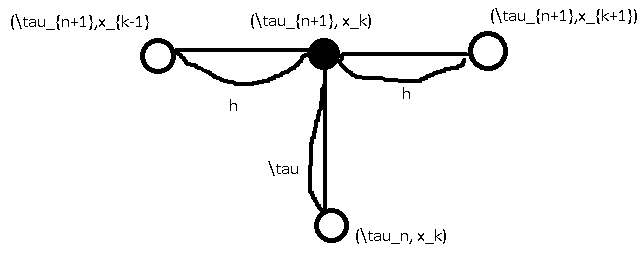
\includegraphics[width=.7\linewidth]{schema}
\end{figure*}

Сетка:
\begin{gather*}
	\begin{cases}
	B\times A,\; B=<0=\tau_0,\tau_1,\cdots,\tau_n>,\; Stp(B)=\tau\\
	A=<hk\;|k\in\mathbb{Z}> \; Stp(A)=h
	\end{cases}
\end{gather*}

Конечно-разностная схема и оператор слоистой структуры:
\begin{gather*}
	\frac{U_k^{n+1}-U_k^n}{\tau}-D\frac{U_{k-1}^{n+1}-2U_{k}^{n+1}+U_{k+1}^{n+1}}{h^2}=0\Rightarrow\\
	U_k^{n+1}-U_k^{n}-D\frac{\tau}{h^2}\left(U_{k-1}^{n+1}-2U_{k}^{n+1}+U_{k+1}^{n+1}\right)=0
\end{gather*}

Оператор слоистой структуры:
\begin{gather*}
U_k^n=e^{ik\theta};\;U_k^{n+1}=\lambda(\theta)e^{ik\theta};\;U_k^n=\lambda^nU_k^0\Rightarrow\\
\lambda-1-D\lambda\frac{\tau}{h^2}(e^{-i\theta}-2+e^{i\theta})=0\Rightarrow
\lambda(\theta)=\frac{1}{1+4D\frac{\tau}{h^2}\sin^2\frac{\theta}{2}}
\end{gather*}

Необходимый спектральный признак устойчивости:
\begin{gather*}
	max\{|\lambda(\theta)|:\theta\in\left[0,2\pi\right]\}=1 \le 1-correct
\end{gather*}
\end{document}
